\subsection{Constructing SCC Tree}

We will look at the construction of the SCC tree for the graph shown in \figureref{\ref{fig:graph1}} by using the algorithm described in the section \secref{\ref{Subsubsec: SCC Tree}}.
We start by finding all the SCCs of the graph and then construct the SCC-Tree for each SCC in it.
This is also used to fill the SCC mapping later used to query the SCC of a node in constant time.\\
Let the example graph be $\mbf{G}$, by running \textsc{find\_scc}($\mbf{G}$) we get SCC(R)


\begin{figure}[H]
    \centering
    \begin{subfigure}{0.45\textwidth}
        \centering
        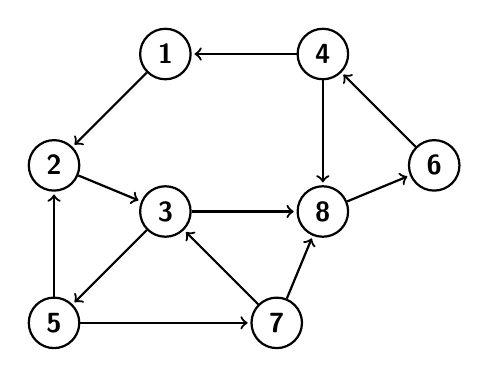
\begin{tikzpicture}[->,shorten >=1pt,auto,node distance=2cm,
            thick,main node/.style={circle,draw,font=\sffamily\bfseries}]

        % Define vertices
        \node[main node] (1) {1};
        \node[main node] (2) [below left of=1] {2};
        \node[main node] (3) [below of=1] {3};
        \node[main node] (4) [right of=1] {4};
        \node[main node] (5) [below left of=3] {5};
        \node[main node] (6) [below right of=4] {6};
        \node[main node] (7) [below right of=3] {7};
        \node[main node] (8) [right of=3] {8};
        

        % Draw edges
        \path[every node/.style={font=\sffamily\small}]
            (1) edge (2)
            (2) edge (3)
            (3) edge (5)
            (3) edge (8)
            (4) edge (1)
            (4) edge (8)
            (5) edge (2)
            (5) edge (7)
            (6) edge (4)
            (7) edge (3)
            (7) edge (8)
            (8) edge (6);

        \end{tikzpicture}
        \caption{Graph 1}
        \label{fig:graph1}
    \end{subfigure}
    \hfill
    \begin{subfigure}{0.45\textwidth}
        \centering
        
\begin{tikzpicture}[->,shorten >=1pt,auto,node distance=2cm,
            thick,main node/.style={circle,draw,font=\sffamily\bfseries}]

        % Define vertices
        \node[main node] (R) {R};

        \end{tikzpicture}
        \caption{condensed graph 1}
        \label{fig:condensed_graph1}
    \end{subfigure}
    \caption{Graph 1 and its condensed graph}
    \label{fig:graph1_and_condensed_graph1}
\end{figure}


\begin{figure}[H]
    \centering
    \begin{subfigure}{0.45\textwidth}
        \centering
        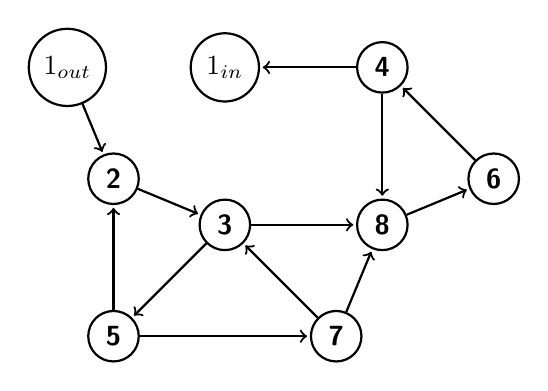
\begin{tikzpicture}[->,shorten >=1pt,auto,node distance=2cm,
            thick,main node/.style={circle,draw,font=\sffamily\bfseries}]

        % Define vertices
        \node[main node] (1) {$1_{in}$};
        \node[main node] (11) [left of=1] {$1_{out}$};
        \node[main node] (2) [below left of=1] {2};
        \node[main node] (3) [below of=1] {3};
        \node[main node] (4) [right of=1] {4};
        \node[main node] (5) [below left of=3] {5};
        \node[main node] (6) [below right of=4] {6};
        \node[main node] (7) [below right of=3] {7};
        \node[main node] (8) [right of=3] {8};
        

        % Draw edges
        \path[every node/.style={font=\sffamily\small}]
            (11) edge (2)
            (2) edge (3)
            (3) edge (5)
            (3) edge (8)
            (4) edge (1)
            (4) edge (8)
            (5) edge (2)
            (5) edge (7)
            (6) edge (4)
            (7) edge (3)
            (7) edge (8)
            (8) edge (6);

        \end{tikzpicture}
        \caption{SCC(R) split on 1}
        \label{fig:scc_r_split}
    \end{subfigure}
    \hfill
    \begin{subfigure}{0.45\textwidth}
        \centering
        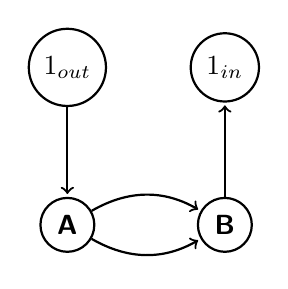
\begin{tikzpicture}[->,shorten >=1pt,auto,node distance=2cm,
            thick,main node/.style={circle,draw,font=\sffamily\bfseries}]

        % Define vertices
        \node[main node] (1) {$1_{in}$};
        \node[main node] (11) [left of=1] {$1_{out}$};
        \node[main node] (A) [below of=11] {A};
        \node[main node] (B) [below of=1] {B};
        

        % Draw edges
        \path[every node/.style={font=\sffamily\small}]
            (11) edge (A)
            (A) edge[bend left] (B)
            (A) edge[bend right] (B)
            (B) edge (1);

        \end{tikzpicture}
        \caption{condensed graph}
        \label{fig:condensed_scc_r_split}
    \end{subfigure}
    \caption{SCC(R) split on 1 and its condensed graph}
    \label{fig:scc_r_split_and_condensed_graph1}
\end{figure}

\begin{figure}[H]
    \centering
    \begin{subfigure}{0.45\textwidth}
        \centering
        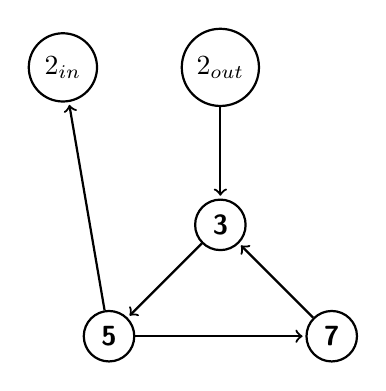
\begin{tikzpicture}[->,shorten >=1pt,auto,node distance=2cm,
            thick,main node/.style={circle,draw,font=\sffamily\bfseries}]

        % Define vertices
        \node[main node] (2) {$2_{out}$};
        \node[main node] (22) [left of=2] {$2_{in}$};
        \node[main node] (3) [below of=2] {3};
        \node[main node] (5) [below left of=3] {5};
        \node[main node] (7) [below right of=3] {7};
        

        % Draw edges
        \path[every node/.style={font=\sffamily\small}]
            (2) edge (3)
            (3) edge (5)
            (5) edge (22)
            (5) edge (7)
            (7) edge (3);

        \end{tikzpicture}
        \caption{SCC(A) split on 2}
        \label{fig:scc_a_split}
    \end{subfigure}
    \hfill
    \begin{subfigure}{0.45\textwidth}
        \centering
        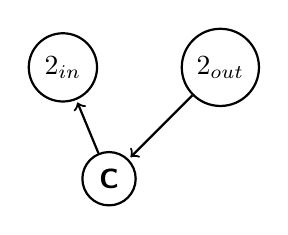
\begin{tikzpicture}[->,shorten >=1pt,auto,node distance=2cm,
            thick,main node/.style={circle,draw,font=\sffamily\bfseries}]

        % Define vertices
        \node[main node] (2) {$2_{out}$};
        \node[main node] (22) [left of=2] {$2_{in}$};
        \node[main node] (C) [below left of=2] {C};
        

        % Draw edges
        \path[every node/.style={font=\sffamily\small}]
            (2) edge (C)
            (C) edge (22);

        \end{tikzpicture}
        \caption{condensed graph}
        \label{fig:condensed_scc_a_split}
    \end{subfigure}
    \caption{SCC(A) split on 2 and its condensed graph}
    \label{fig:scc_a_split_and_condensed_graph1}
\end{figure}

\begin{figure}[H]
    \centering
    \begin{subfigure}{0.45\textwidth}
        \centering
        \begin{tikzpicture}[->,shorten >=1pt,auto,node distance=2cm,
            thick,main node/.style={circle,draw,font=\sffamily\bfseries}]

        % Define vertices
        \node[main node] (4) {$4_{in}$};
        \node[main node] (44) [left of=1] {$4_{out}$};
        \node[main node] (6) [below of=1] {6};
        \node[main node] (8) [below of=11] {8};
        

        % Draw edges
        \path[every node/.style={font=\sffamily\small}]
            (44) edge (8)
            (8) edge (6)
            (6) edge (4);

        \end{tikzpicture}
        \caption{SCC(B) split on 4}
        \label{fig:scc_b_split}
    \end{subfigure}
    \hfill
    \begin{subfigure}{0.45\textwidth}
        \centering
        \begin{tikzpicture}[->,shorten >=1pt,auto,node distance=2cm,
            thick,main node/.style={circle,draw,font=\sffamily\bfseries}]

        % Define vertices
        \node[main node] (4) {$4_{in}$};
        \node[main node] (44) [left of=1] {$4_{out}$};
        \node[main node] (6) [below of=1] {6};
        \node[main node] (8) [below of=11] {8};
        

        % Draw edges
        \path[every node/.style={font=\sffamily\small}]
            (44) edge (8)
            (8) edge (6)
            (6) edge (4);

        \end{tikzpicture}
        \caption{condensed graph}
        \label{fig:condensed_scc_b_split}
    \end{subfigure}
    \caption{SCC(B) split on 4 and its condensed graph}
    \label{fig:scc_b_split_and_condensed_graph1}
\end{figure}

\begin{figure}[H]
    \centering
    \begin{subfigure}{0.45\textwidth}
        \centering
        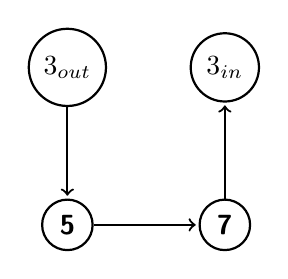
\begin{tikzpicture}[->,shorten >=1pt,auto,node distance=2cm,
            thick,main node/.style={circle,draw,font=\sffamily\bfseries}]

        % Define vertices
        \node[main node] (3) {$3_{in}$};
        \node[main node] (33) [left of=3] {$3_{out}$};
        \node[main node] (5) [below of=33] {5};
        \node[main node] (7) [below of=3] {7};
        

        % Draw edges
        \path[every node/.style={font=\sffamily\small}]
            (33) edge (5)
            (5) edge (7)
            (7) edge (3);

        \end{tikzpicture}
        \caption{SCC(C) split on 3}
        \label{fig:scc_c_split}
    \end{subfigure}
    \hfill
    \begin{subfigure}{0.45\textwidth}
        \centering
        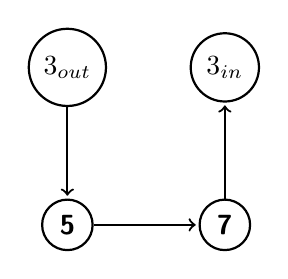
\begin{tikzpicture}[->,shorten >=1pt,auto,node distance=2cm,
            thick,main node/.style={circle,draw,font=\sffamily\bfseries}]

        % Define vertices
        \node[main node] (3) {$3_{in}$};
        \node[main node] (33) [left of=3] {$3_{out}$};
        \node[main node] (5) [below of=33] {5};
        \node[main node] (7) [below of=3] {7};
        

        % Draw edges
        \path[every node/.style={font=\sffamily\small}]
            (33) edge (5)
            (5) edge (7)
            (7) edge (3);

        \end{tikzpicture}
        \caption{condensed graph}
        \label{fig:condensed_scc_c_split}
    \end{subfigure}
    \caption{SCC(C) split on 3 and its condensed graph}
    \label{fig:scc_c_split_and_condensed_graph1}
\end{figure}

\begin{figure}[H]
    \centering
    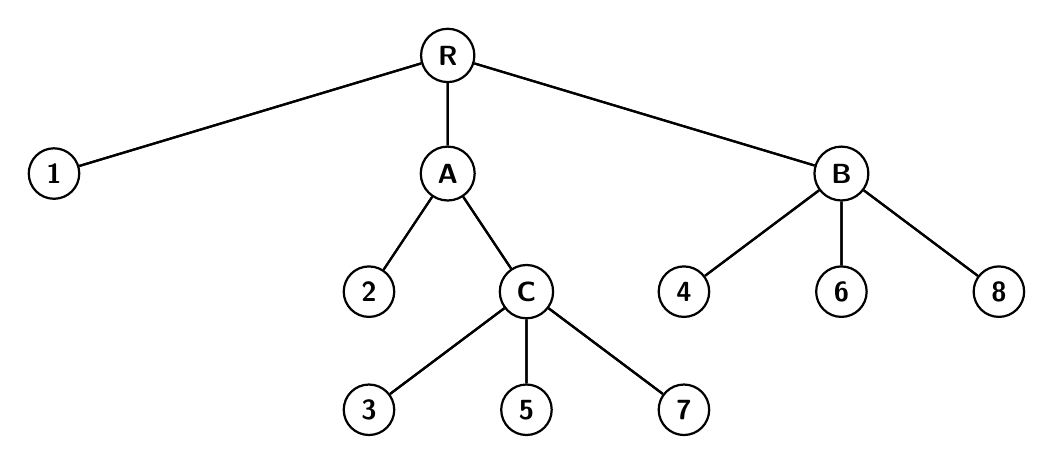
\begin{tikzpicture}[level distance=1.5cm,
                        level 1/.style={sibling distance=5cm},
                        level 2/.style={sibling distance=2cm},
                        thick,main node/.style={circle,draw,font=\sffamily\bfseries}]

      % Define vertices
      \node[main node] (R) {R}
        child {node[main node] (1) {1}}
        child {node[main node] (A) {A}
          child {node[main node] (2) {2}}
          child {node[main node] (C) {C}
            child {node[main node] (3) {3}}
            child {node[main node] (5) {5}}
            child {node[main node] (7) {7}}
          }
        }
        child {node[main node] (B) {B}
          child {node[main node] (4) {4}}
          child {node[main node] (6) {6}}
          child {node[main node] (8) {8}}
        };

      % Draw edges
      \path[every node/.style={font=\sffamily\small}]
        (R) edge (1)
        (R) edge (A)
        (R) edge (B)
        (A) edge (2)
        (A) edge (C)
        (B) edge (4)
        (B) edge (6)
        (B) edge (8)
        (C) edge (3)
        (C) edge (5)
        (C) edge (7);

    \end{tikzpicture}
    \caption{SCC Tree of Graph \ref{fig:graph1}}
    \label{fig:scc_tree_graph1}
\end{figure}

